\documentclass[../main.tex]{subfiles}
\graphicspath{{\subfix{../../img/}}}
\begin{document}


\newpage
\section{Prototyping}

In diesem Abschnitt werden für bestimmte Teilbereiche ein Prototyp erstellt,
um Risikos aus der Risikoanalyse (siehe \ref{risikomatrix}) zu minimieren.

\subsection{Objekterkennung}

Unser Team hat noch keine Erfahrung mit Bild- beziehungsweise Objekterkennung.
Dies ist ein sehr komplexes Thema, weshalb es ein Risiko darstellt.
Damit wir bereits früh erste Erfahrungen sammeln können, haben wir deshalb bereits in PREN-1 mit einem Prototypen zur Objekterkennung begonnen.

Um ein Objekterkennungsmodell zu trainieren, braucht es viele Bilder von den Objekten, die man erkennen will. Bei uns sind das Wegpunkte, Pylonen und Hindernisse.

Deshalb haben wir in der Mensa, wo der Wettbewerb stattfinden wird, den Graphen mit den spezifizierten Wegpunkten und Klebeband aufgeklebt. Darauf platzierten wir eine Pylone sowie ein Hindernis an verschiedenen Orten und machten viele Bilder aus ungefähr 30 Zentimetern Höhe.

Hier sind einige Beispiel für

\begin{center}
\begin{figure}[H]
\begin{tabular}{cc}
    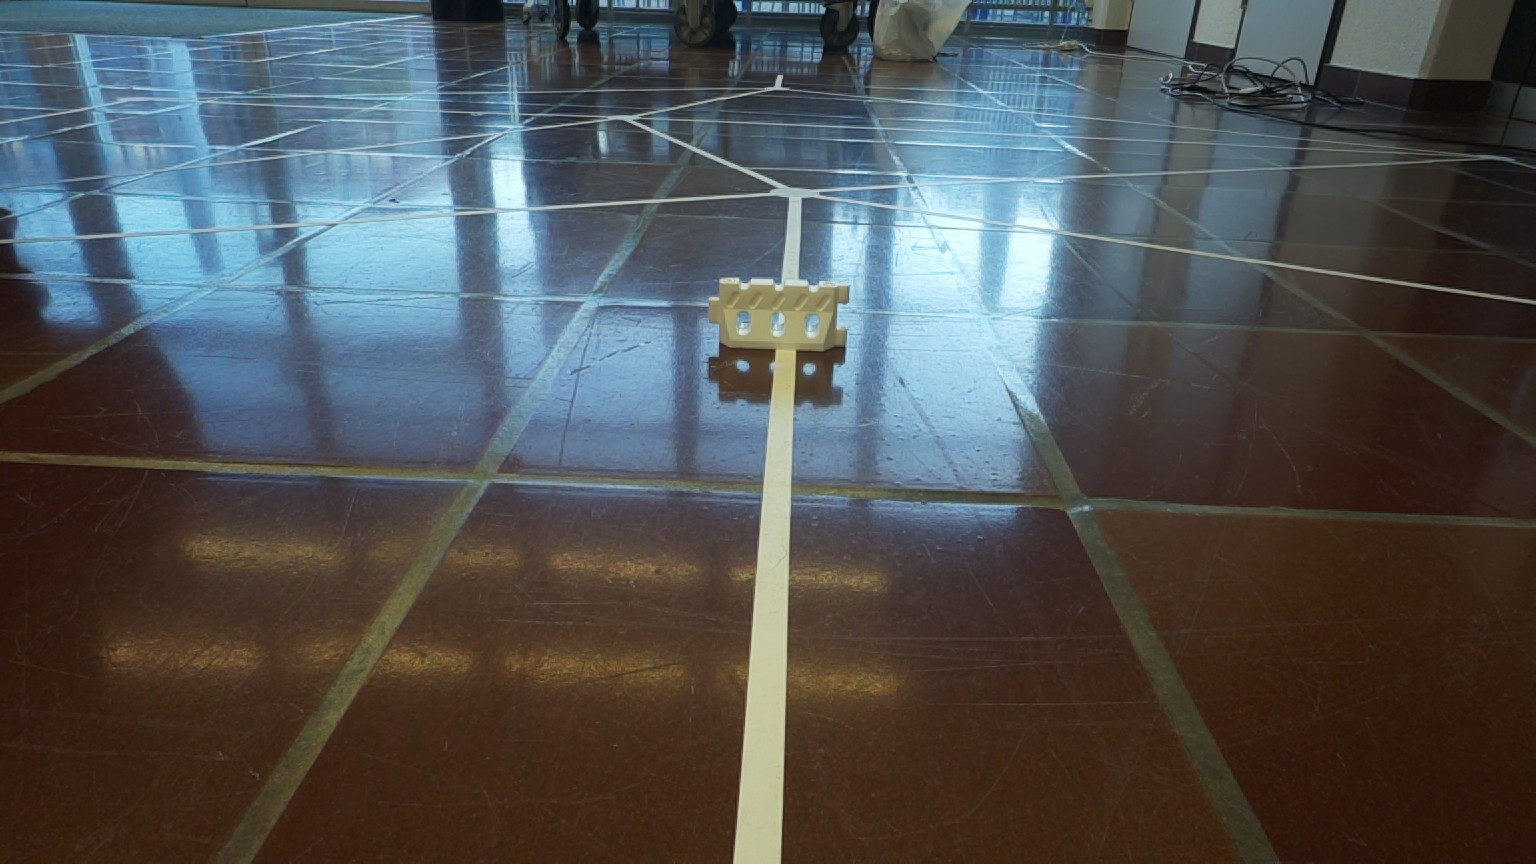
\includegraphics[width=0.5\textwidth]{img/prototyping/objekterkennung/Bild1.jpg} &
    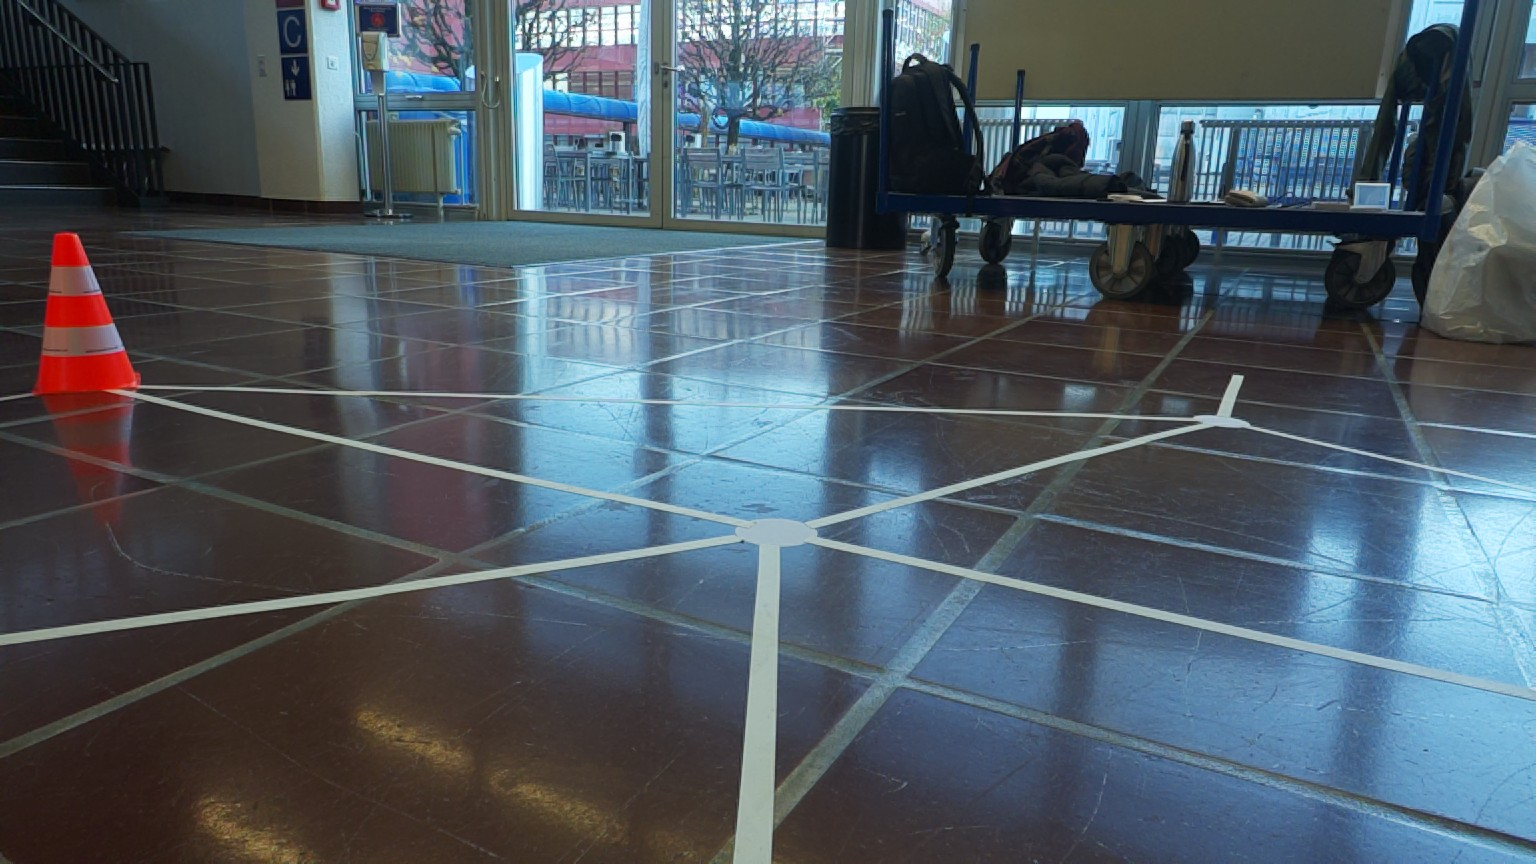
\includegraphics[width=0.5\textwidth]{img/prototyping/objekterkennung/Bild2.jpg} \\
    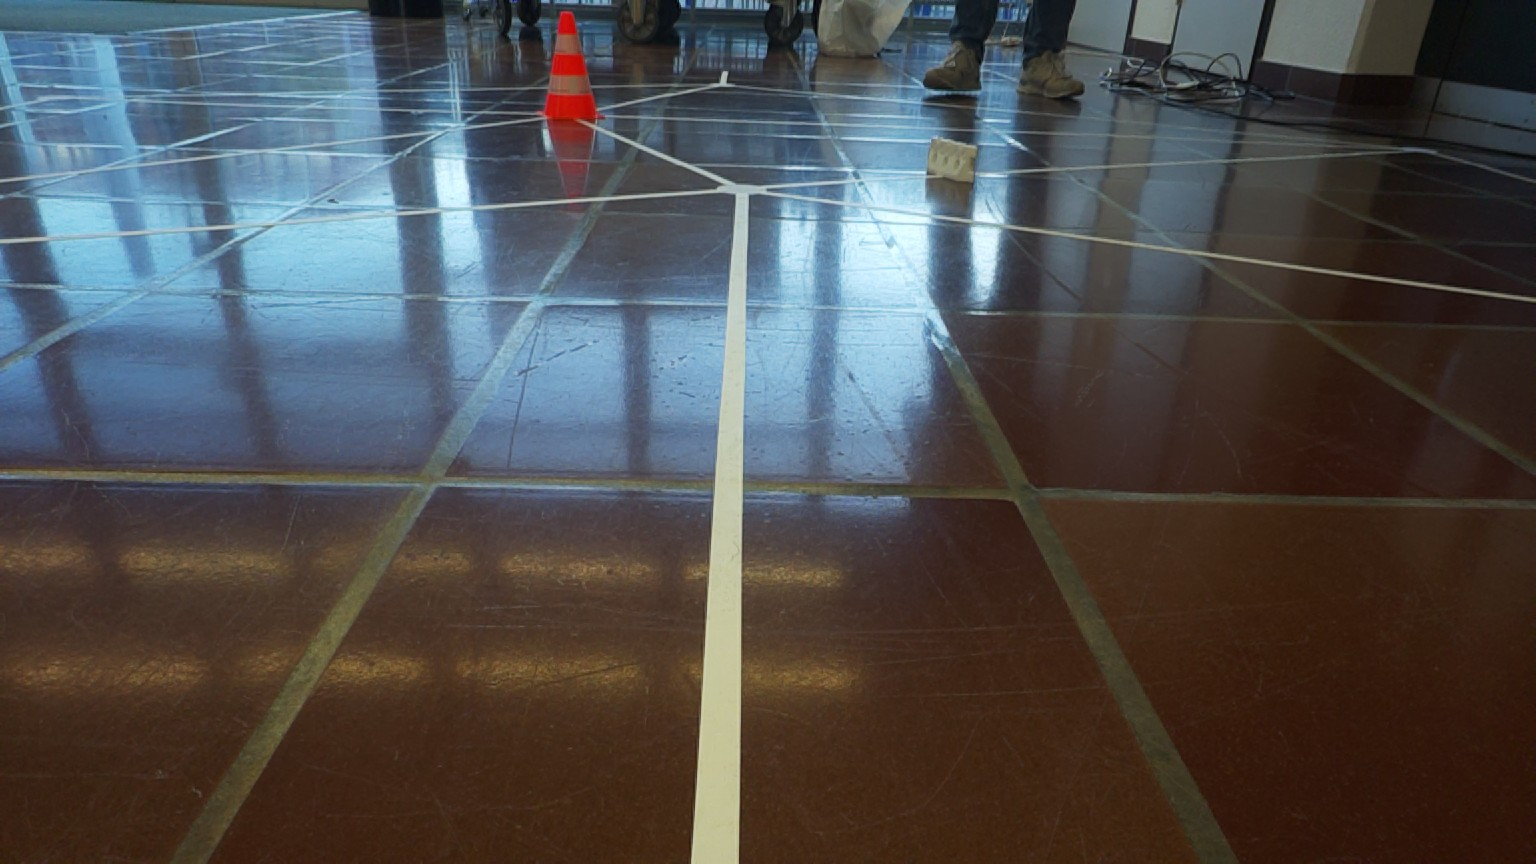
\includegraphics[width=0.5\textwidth]{img/prototyping/objekterkennung/Bild3.jpg} &
    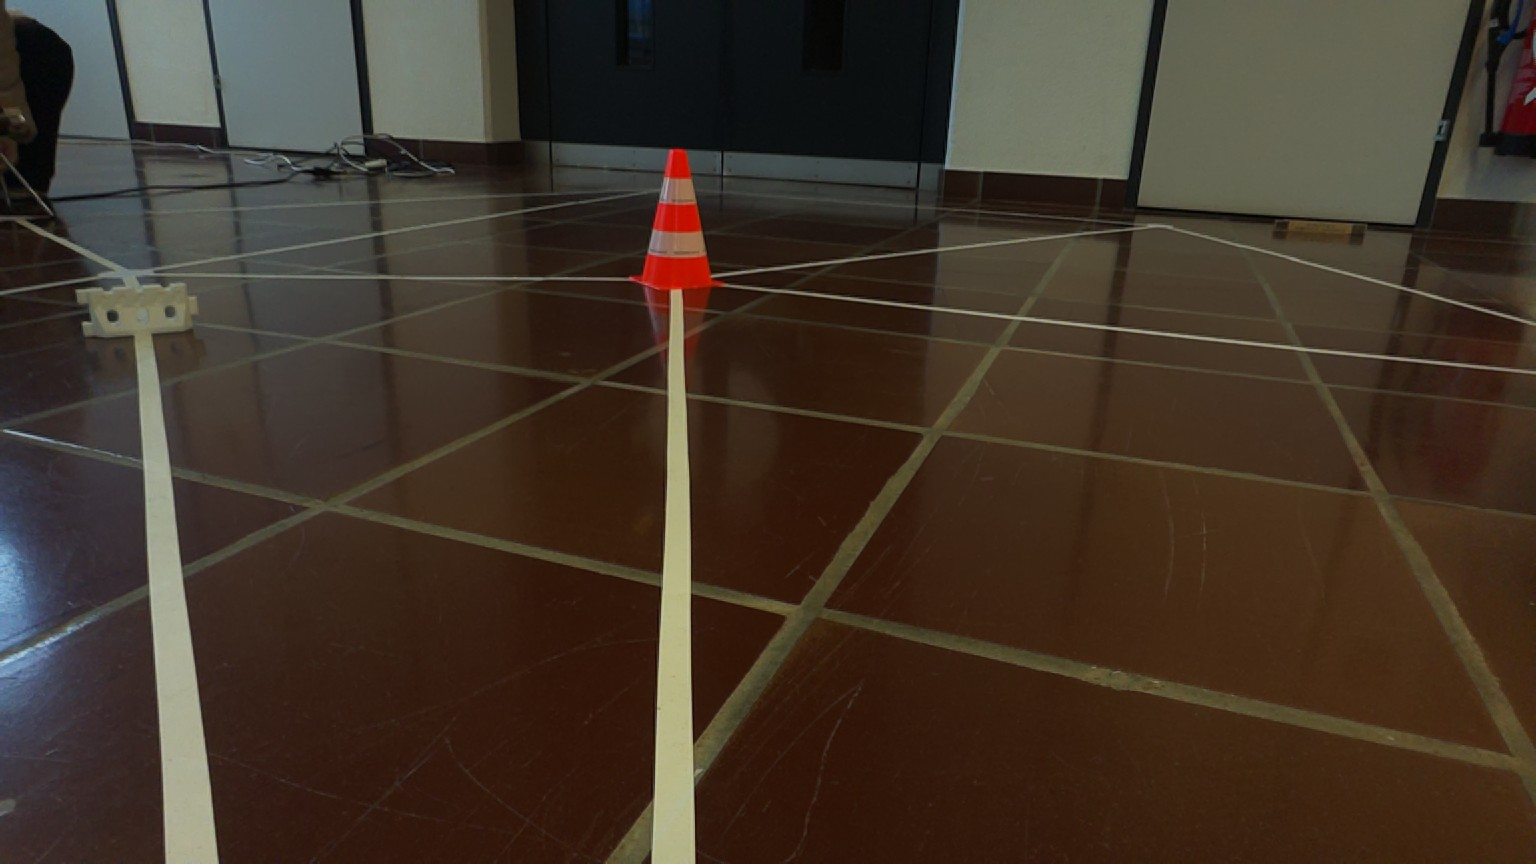
\includegraphics[width=0.5\textwidth]{img/prototyping/objekterkennung/Bild4.jpg}
\end{tabular}
\caption{Bilder für den Objekterkennungs-Prototypen}
\end{figure}
\end{center}

\end{document}